\chapter{Perancangan}
\label{chap:perancangan}

\section{Diagram Kelas Rinci} 
\label{sec:diagram_kelas_rinci}
Diagram kelas rinci diperoleh dari hasil pengembangan diagram kelas analisis pada subbab \ref{sec:analisis_kelas}. Diagram kelas rinci dapat dilihat pada Gambar \ref{fig:4_final_class_diagram}. 
	\begin{figure}[ht]
			\centering
			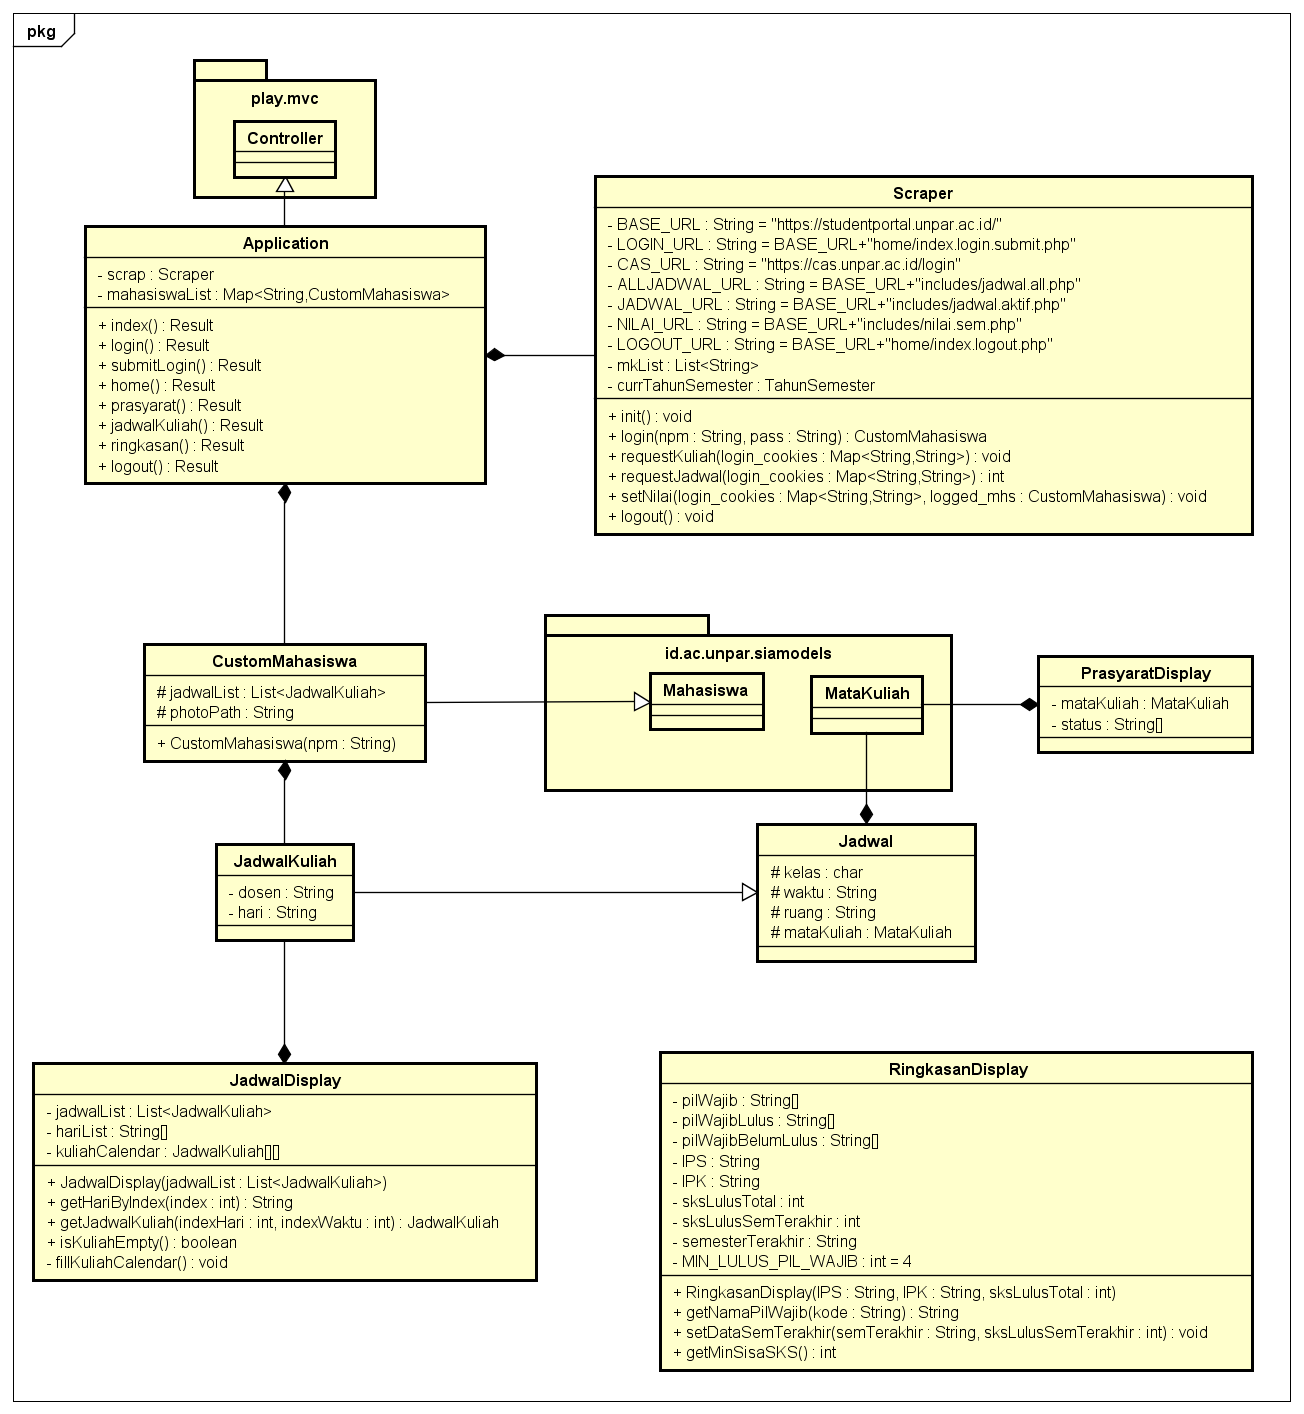
\includegraphics[scale=0.45]{Gambar/class-diagram-final}
			\caption{Diagram Kelas Rinci} 
			\label{fig:4_final_class_diagram}
		\end{figure}
	Deskripsi kelas beserta fungsi dari diagram kelas rinci tersebut adalah sebagai berikut:
	\begin{enumerate}
		\item Application\\
		Kelas ini merupakan turunan dari kelas Controller yang dimiliki oleh Play Framework sehingga menjadikan kelas ini sebagai controller dari aplikasi Informatika Student Portal. Atribut yang dimiliki kelas ini antara lain:
		\begin{itemize}
			\item \textbf{Scraper scrap:} objek Scraper yang berperan dalam pengambilan data dari Porta Akademik Mahasiswa.
			\item \textbf{Map<String,CustomMahasiswa> mahasiswaList:} kumpulan objek Mahasiswa merepresentasikan mahasiswa yang sedang menggunakan aplikasi.
		\end{itemize}
	\textit{Method-method} yang dimiliki kelas ini merupakan \textit{action method} dengan rincian sebagai berikut:
		\begin{itemize}
			
			\item \textbf{public Result index()}\\
				Berfungsi untuk mengarahkan pengguna ke halaman Informatika Student Portal.\\
				\textbf{Kembalian:} halaman \textit{login} jika pengguna belum \textit{login} atau halaman utama jika pengguna sudah \textit{login}.
				
			\item \textbf{public Result login()}\\
				Berfungsi untuk mengarahkan pengguna ke halaman \textit{login}.\\
				\textbf{Kembalian:} halaman \textit{login} jika pengguna belum \textit{login} atau halaman utama jika pengguna sudah \textit{login}.
				
			\item \textbf{public Result submitLogin()}\\
				Berfungsi untuk mengirimkan data dari halaman \textit{login} sekaligus melakukan validasi akun.\\
				\textbf{Kembalian:} halaman utama jika \textit{login} berhasil atau halaman \textit{login} jika \textit{login} gagal.
				
			\item \textbf{public Result home()}\\
				Berfungsi untuk mengarahkan pengguna ke halaman utama.\\
				\textbf{Kembalian:} halaman utama.
				
			\item \textbf{public Result prasyarat()}\\
				Berfungsi untuk mengarahkan pengguna ke halaman prasyarat mata kuliah.\\
				\textbf{Kembalian:} halaman prasyarat mata kuliah.
				
			\item \textbf{public Result jadwalKuliah()}\\
				Berfungsi untuk mengarahkan pengguna ke halaman jadwal kuliah.\\
				\textbf{Kembalian:} halaman jadwal kuliah.
				
			\item \textbf{public Result ringkasan()}\\
				Berfungsi untuk mengarahkan pengguna ke halaman ringkasan data akademik.\\
				\textbf{Kembalian:} halaman ringkasan data akademik.
				
			\item \textbf{public Result logout()}\\
				Berfungsi untuk mengeluarkan pengguna yang sedang \textit{login}.\\
				\textbf{Kembalian:} halaman \textit{login}.
		\end{itemize}
		
		\item Scaper\\
		Kelas ini mengimplementasikan \textit{library} jsoup untuk melakukan pengambilan data dari Portal Akademik Mahasiswa. Atribut yang dimiliki kelas ini antara lain:
		\begin{itemize}
			\item \textbf{String BASE\_URL:} URL Portal Akademik Mahasiswa.
			\item \textbf{String LOGIN\_URL:} URL \textit{login} Portal Akademik Mahasiswa.
			\item \textbf{String CAS\_URL:} URL \textit{login} CAS UNPAR.
			\item \textbf{String ALLJADWAL\_URL:} URL jadwal seluruh fakultas pada Portal Akademik Mahasiswa.
			\item \textbf{String JADWAL\_URL:} URL jadwal mahasiswa pada Portal Akademik Mahasiswa.
			\item \textbf{String NILAI\_URL:} URL riwayat nilai mahasiswa pada Portal Akademik Mahasiswa.
			\item \textbf{String LOGOUT\_URL:} URL \textit{logout} Portal Akademik Mahasiswa.
			\item \textbf{TahunSemester currTahunSemester:} tahun ajaran dan semester terkini.
			\item \textbf{List<MataKuliah> mkList:} daftar mata kuliah yang dibuka pada semester terkini.
		\end{itemize}
	\textit{Method-method} yang dimiliki kelas ini adalah sebagai berikut:
		\begin{itemize}
			\item \textbf{public void init()}\\
			Berfungsi untuk menginisialisasi koneksi ke Portal Akademik Mahasiswa.\\
			\textbf{Kembalian:} tidak ada.
			
			\item \textbf{public CustomMahasiswa login(String npm, String pass)}\\
				Berfungsi untuk melakukan \textit{login}.\\
				\textbf{Parameter:}
				\begin{itemize}
					\item \textbf{npm} NPM mahasiswa.
					\item \textbf{pass} \textit{password} mahasiswa.
				\end{itemize}
				\textbf{Kembalian:} objek Mahasiswa.

			\item \textbf{public void requestKuliah(Map<String,String> login\_cookies)}\\
				Berfungsi untuk mendapatkan daftar mata kuliah yang dibuka pada semester terkini.\\
				\textbf{Parameter:}
				\begin{itemize}
					\item \textbf{login\_cookies} \textit{cookie} mahasiswa yang telah \textit{login}.
				\end{itemize}
				\textbf{Kembalian:} tidak ada.
				
			\item \textbf{public List<JadwalKuliah> requestJadwal(Map<String,String> login\_cookies)}\\
				Berfungsi untuk mendapatkan jadwal kuliah mahasiswa pada semester terkini.\\
				\textbf{Parameter:}
				\begin{itemize}
					\item \textbf{login\_cookies} \textit{cookie} mahasiswa yang telah \textit{login}.
				\end{itemize}
				\textbf{Kembalian:} jadwal kuliah mahasiswa pada semester terkini.
				
			\item \textbf{public void setNilai(Map<String,String> login\_cookies, Mahasiswa logged\_mhs)}\\
				Berfungsi untuk mendapatkan riwayat nilai mahasiswa.\\
				\textbf{Parameter:}
				\begin{itemize}
					\item \textbf{login\_cookies} \textit{cookie} mahasiswa yang telah \textit{login}.
					\item \textbf{logged\_mhs} objek Mahasiswa dari mahasiswa yang telah \textit{login}.
				\end{itemize}
				\textbf{Kembalian:} tidak ada.
			
			\item \textbf{public void logout()}\\
				Berfungsi untuk melakukan \textit{logout}.\\
				\textbf{Kembalian:} tidak ada.
		\end{itemize}
		
		\item CustomMahasiswa\\
		Kelas ini merupakan turunan dari kelas Mahasiswa. Kelas ini merepresentasikan mahasiswa yang memiliki jadwal kuliah dan URL foto profil. Atribut yang dimiliki kelas ini antara lain:
		\begin{itemize}
			\item \textbf{String photoPath:}  URL foto profil mahasiswa pada Portal Akademik Mahasiswa.
			\item \textbf{List<JadwalKuliah> jadwalList:} daftar jadwal kuliah mahasiswa.
		\end{itemize}
	\textit{Method-method} yang dimiliki kelas ini adalah sebagai berikut:
		\begin{itemize}
			\item \textbf{public CustomMahasiswa(String npm)}\\
			Merupakan \textit{constructor} dari kelas CustomMahasiswa.\\
			\textbf{Parameter:}
			\begin{itemize}
				\item \textbf{npm} Nomor Pokok Mahasiswa.
			\end{itemize}
		\end{itemize}
		
		\item Jadwal\\
		Kelas ini merepresentasikan jadwal di UNPAR. Atribut yang dimiliki kelas ini antara lain:
		\begin{itemize}
			\item \textbf{MataKuliah mataKuliah:} mata kuliah.
			\item \textbf{char kelas:} kelas kuliah.
			\item \textbf{String waktu:} waktu pelaksanaan kuliah.
			\item \textbf{String ruang:} ruang kuliah.
		\end{itemize}
		
		\item JadwalKuliah\\
		Kelas ini merepresentasikan jadwal di UNPAR. Atribut yang dimiliki kelas ini antara lain:
		\begin{itemize}
			\item \textbf{MataKuliah mataKuliah:} mata kuliah.
			\item \textbf{char kelas:} kelas kuliah.
			\item \textbf{String waktu:} waktu pelaksanaan kuliah.
			\item \textbf{String ruang:} ruang kuliah.
		\end{itemize}
		
		\item PrasyaratDisplay\\
		Kelas berfungsi sebagai media pengiriman data ke halaman prasyarat mata kuliah. Atribut yang dimiliki kelas ini antara lain:
		\begin{itemize}
			\item \textbf{MataKuliah mataKuliah:} mata kuliah.
			\item \textbf{String[] status:} status pengambilan mata kuliah.
		\end{itemize}
		
		\item JadwalDisplay\\
		Kelas berfungsi sebagai media pengiriman data ke halaman jadwal mata kuliah. Atribut yang dimiliki kelas ini antara lain:
		\begin{itemize}
			\item \textbf{JadwalKuliah[][] kuliahCalendar:} jadwal kuliah mahasiswa dalam \textit{array}.
			\item \textbf{String[] hariList:} nama-nama hari dalam String.
			\item \textbf{List<JadwalKuliah> jadwalList:} daftar jadwal kuliah mahasiswa.
		\end{itemize}
	\textit{Method-method} yang dimiliki kelas ini adalah sebagai berikut:
		\begin{itemize}
			\item \textbf{public JadwalDisplay(List<JadwalKuliah> jadwalList)}\\
			Merupakan \textit{constructor} dari kelas JadwalDisplay.\\
			\textbf{Parameter:}
			\begin{itemize}
				\item \textbf{jadwalList} jadwal kuliah mahasiswa.
			\end{itemize}
			
			\item \textbf{public String getHariByIndex(int index)}\\
				Berfungsi untuk mendapatkan hari berdasarkan angka index. Angka index dimulai dari 0 sedangkan hari dimulai dari Senin.\\
				\textbf{Parameter:}
				\begin{itemize}
					\item \textbf{index} angka index hari.
				\end{itemize}
				\textbf{Kembalian:} hari dalam String.
		
		\item \textbf{public JadwalKuliah getJadwalKuliah(int indexHari, int indexWaktu)}\\
				Berfungsi untuk mendapatkan jadwal kuliah dari atribut kuliahCalendar.\\
				\textbf{Parameter:}
				\begin{itemize}
					\item \textbf{indexHari} angka index hari.
					\item \textbf{indexWaktu} angka index waktu.
				\end{itemize}
				\textbf{Kembalian:} jadwal kuliah.
		
		\item \textbf{public boolean isKuliahEmpty()}\\
				Berfungsi untuk memeriksa apakah nilai dari jadwal kuliah kosong.\\
				\textbf{Kembalian:} \texttt{true} jika kosong, \texttt{false} jika tidak kosong.
		
		\item \textbf{private void fillKuliahCalendar()}\\
				Berfungsi untuk mengisi atribut kuliahCalendar berdasarkan atribut jadwalList.\\
				\textbf{Kembalian:} tidak ada.
		\end{itemize}
		
				\item RingkasanDisplay\\
		Kelas berfungsi sebagai media pengiriman data ke halaman ringkasan data akademik. Atribut yang dimiliki kelas ini antara lain:
		\begin{itemize}
			\item \textbf{String[] pilWajib:} kode-kode mata kuliah pilihan wajib.
			\item \textbf{String[] pilWajibLulus:} kode-kode mata kuliah pilihan wajib yang sudah lulus.
			\item \textbf{String[] pilWajibBelumLulus:} kode-kode mata kuliah pilihan wajib yang belum lulus.
			\item \textbf{String IPS:} IPS mahasiswa.
			\item \textbf{String IPK:} IPK mahasiswa.
			\item \textbf{String semesterTerakhir:} semester terakhir yang telah ditempuh mahasiswa.
			\item \textbf{int sksLulusTotal:} total sks lulus mahasiswa.
			\item \textbf{int sksLulusSemTerakhir:} sks lulus mahasiswa pada semester terakhir.
			\item \textbf{int MIN\_LULUS\_PIL\_WAJIB:} banyaknya mata kuliah pilihan wajib minimum untuk kelulusan dengan nilai 4.
		\end{itemize}
		\textit{Method-method} yang dimiliki kelas ini adalah sebagai berikut:
		\begin{itemize}
			\item \textbf{public RingkasanDisplay(String IPS, String IPK, int sksLulusTotal)}\\
			Merupakan \textit{constructor} dari kelas Ringkasan Display.\\
			\textbf{Parameter:}
			\begin{itemize}
				\item \textbf{IPS} IPS mahasiswa.
				\item \textbf{IPK} IPK mahasiswa.
				\item \textbf{sksLulusTotal} total sks lulus mahasiswa.
			\end{itemize}
			
			\item \textbf{public String getNamaPilWajib(String kode)}\\
				Berfungsi untuk mendapatkan nama mata kuliah pilihan wajib.\\
				\textbf{Parameter:}
					\begin{itemize}
						\item \textbf{kode} kode mata kuliah pilihan wajib.
					\end{itemize}
				\textbf{Kembalian:} nama mata kuliah pilihan wajib.

			\item \textbf{public void setDataSemTerakhir(String semTerakhir, int sksLulusSemTerakhir)}\\
				Berfungsi untuk mengisi data semester terakhir.\\
				\textbf{Parameter:}
				\begin{itemize}
					\item \textbf{semTerakhir} semester terakhir yang telah ditempuh mahasiswa.
					\item \textbf{sksLulusSemTerakhir} sks lulus mahasiswa pada semester terakhir.
				\end{itemize}
				\textbf{Kembalian:} tidak ada.
				
				\item \textbf{public int getMinSisaSKS()}\\
				Berfungsi untuk mendapatkan sisa sks minimum untuk kelulusan.\\
				\textbf{Kembalian:} sisa sks untuk minimum kelulusan.
		\end{itemize}
		
	\end{enumerate}

\section{Perancangan Antarmuka}
\label{sec:perancangan_antarmuka}

Untuk memenuhi kebutuhan interaksi antara pengguna dengan sistem, maka dirancanglah sebuah antarmuka dari Informatika Student Portal. Rancangan antarmuka dibagi menjadi lima halaman web antara lain:

\begin{enumerate}
	\item {Antarmuka Halaman \textit{Login}}\\
	Halaman ini digunakan untuk melakukan \textit{login}. Komponen halaman ini terdiri dari logo aplikasi, kolom \textit{email}, kolom \textit{password}, dan tombol \textit{login} seperti yang ditunjukkan pada Gambar \ref{fig:4_ranc_login}. Untuk melakukan \textit{login}, pengguna perlu memasukkan \textit{email} dan \textit{password} yang sesuai kemudian menekan tombol \textit{login}. Jika berhasil pengguna akan diarahkan ke halaman \textit{home}. 
		\begin{figure}[H]
			\centering
			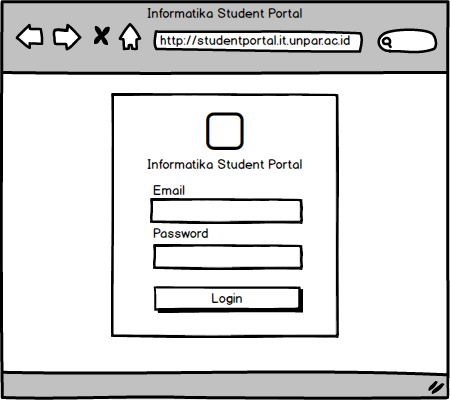
\includegraphics[scale=0.5]{Gambar/Login_Page}
			\caption{Rancangan Halaman \textit{Login}} 
			\label{fig:4_ranc_login}
		\end{figure}
		
	\item {Antarmuka Halaman \textit{Home}}\\
	Halaman \textbf{home} merupakan halaman yang pertama dituju setelah melakukan \textbf{login}. Halaman ini, menampilkan identitas pengguna seperti foto profil, nama, Nomor Induk Mahasiswa(NPM), dan \textit{email} mahasiswa. Rancangan antarmuka halaman \textit{home} dapat dilihat pada Gambar \ref{fig:4_ranc_home}.
		\begin{figure}[H]
			\centering
			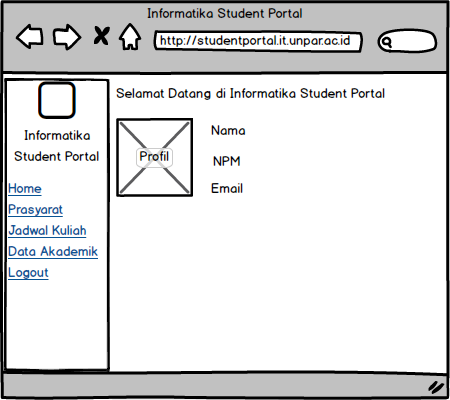
\includegraphics[scale=0.5]{Gambar/Home_Page}
			\caption{Rancangan Halaman \textit{Home}} 
			\label{fig:4_ranc_home}
		\end{figure}
		
	\item {Antarmuka Halaman Prasyarat Mata Kuliah}\\
	Halaman ini menampilkan tabel prasyarat mata kuliah yang dibuka pada semester terkini. Tabel tersebut memiliki tiga kolom yaitu kode mata kuliah, nama mata kuliah, dan status pengambilan mata kuliah. Rancangan antarmuka halaman prasyarat mata kuliah dapat dilihat pada Gambar \ref{fig:4_ranc_prasyarat}.
	\begin{figure}[H]
			\centering
			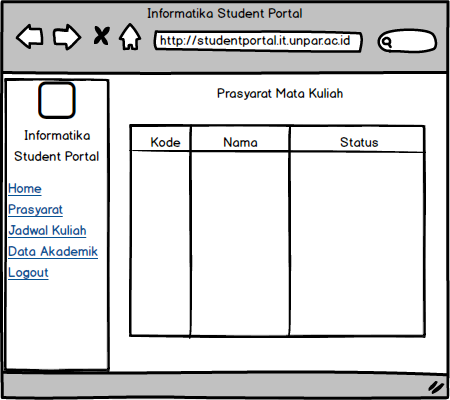
\includegraphics[scale=0.5]{Gambar/Prasyarat_Page}
			\caption{Rancangan Halaman Prasyarat Mata Kuliah} 
			\label{fig:4_ranc_prasyarat}
		\end{figure}
	\item {Antarmuka Halaman Jadwal Kuliah}\\
	Halaman ini menampilkan jadwal kuliah semester terkini yang tersusun dan terurut berdasarkan hari. Rancangan antarmuka halaman jadwal kuliah dapat dilihat pada Gambar \ref{fig:4_ranc_kuliah}.
	\begin{figure}[H]
			\centering
			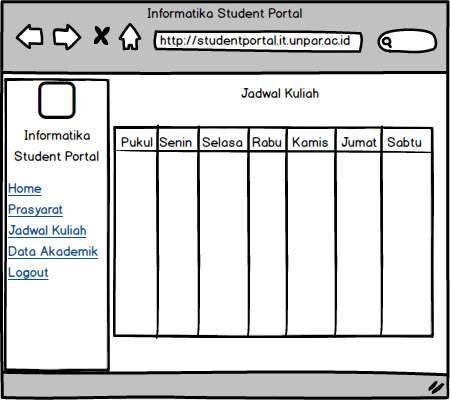
\includegraphics[scale=0.5]{Gambar/Jadwal_Page}
			\caption{Rancangan Halaman Jadwal Kuliah} 
			\label{fig:4_ranc_kuliah}
		\end{figure}
	\item {Antarmuka Halaman Data Akademik}\\
	Halaman ini menampilkan ringkasan informasi akademik pengguna yaitu IPS semester terakhir, IPK, SKS lulus, sisa SKS menuju kelulusan, dan status pengambilan mata kuliah pilihan wajib. Rancangan antarmuka halaman data akademik dapat dilihat pada Gambar \ref{fig:4_ranc_ringkasan}.
	\begin{figure}[H]
			\centering
			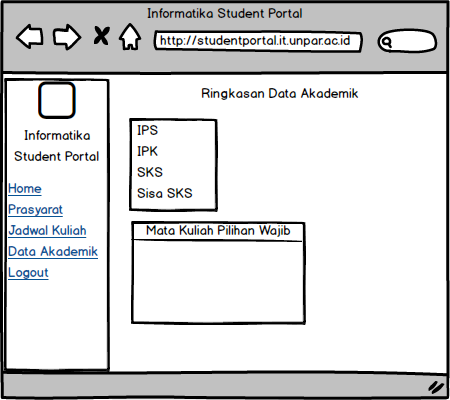
\includegraphics[scale=0.5]{Gambar/Ringkasan_Page}
			\caption{Rancangan Halaman Data Akademik} 
			\label{fig:4_ranc_ringkasan}
		\end{figure}
\end{enumerate}
